\documentclass[11pt]{article}
%Gummi|065|=)
\title{Homework \#3: Discussion on $k$-means Clustering\\ of CNN News Articles}
\author{Doug McGeehan\\
		CS 6001: Applied Spatial and \\ Temporal Data Analysis\\
		Spring 2017}

\usepackage[margin=1in]{geometry}
\usepackage{verbatim}
\usepackage{framed}
\usepackage{amsmath}
\usepackage{amssymb}
\usepackage{graphicx}
\usepackage{caption}
\usepackage{subcaption}

\begin{document}

\maketitle

\section{Introduction}

\section{Preliminaries}

Prior to discussing the experimental results, the preliminary concepts and methods used for the experiments are discussed.

\subsection{Feature Subset Selection} \label{sec:feature_selection}

Without performing any feature reduction to the dataset, there exists 11,372 unique terms within the selected 100 articles.
With this high-dimensionality of the dataset, initial executions of $k$-means were found to produce very poor quality clusters.
Thus, it is of interest to perform various methods of dimensionality reduction so as to investigate its effect on the clustering results.
For this report, five feature selection methods were chosen to compare against a benchmark approach: average tf-idf scores, Gini index splitting scores, pairwise feature correlations, feature-to-category correlation, and random forest feature importances, with the benchmark being only the removal of stopwords from each article.
Each of these methods produces a set of features that are preserved in the dataset for executing $k$-means while removing other features deemed ill-suited for representing the articles.
Each of these methods is briefly discussed in the following subsections.

\subsubsection{Feature Selection from Average Tf-idf Scores}

Each article in the dataset may have a distinct tf-idf score for a particular feature.
Some articles may have a score of 0, while others have a significantly larger score.
To perform feature selection, first the tf-idf scores for each feature is averaged over all articles.
Then, these features are ranked in descending order of their average tf-idf score.
Table 1 shows the top 10 features with the highest average tf-idf scores.
From this ordering, feature selection is accomplished by preserving the top $n$ features in the dataset as inputs to the $k$-means algorithm.
All other features are removed.

\begin{center}
\begin{tabular}{ |r|l| } 
 \hline
 Term & Average Tf-idf \\
 \hline
 perez       &   0.7905 \\
 planets     &   0.6817 \\
 chemicals   &   0.6701 \\
 flappy      &   0.6590 \\
 barbie      &   0.6166 \\
 zimmerman   &   0.6023 \\
 cosby       &   0.5690 \\
 colonel     &   0.5684 \\
 meyers      &   0.5568 \\
 sparks      &   0.5457 \\ 
 \hline
\end{tabular}
\end{center}

\subsubsection{Feature Selection from Gini Indexes}

The Gini index approach exploits the process of building decision trees to select high-scoring features.
As a decision tree is being constructed, each node is assigned an attribute that is used to route an object to be classified through the tree.
The manner in which an attribute is selected for a node is determined based on the reduction of impurity that is achieved by from partitioning articles on the attribute's value in each article.
Should the splitting on one attribute result in the lowest impurity of each of the partitions, then that attribute is selected for the node being constructed within the decision tree.
There are multiple impurity metrics that could be selected, as was investigated in the previous report.
For this report, the Gini index was chosen.

To adapt this process for feature subset selection, each feature is assigned the impurity score obtained by partitioning the dataset on that attribute's observed values.
For a given feature, the dataset is split into two partitions, with one consisting of the articles exhibiting a tf-idf score less than some threshold.
All other articles are within the second partition, exhibiting tf-idf scores greater than or equal to the threshold.
The threshold is chosen based on which tf-idf value offers the lowest Gini index by the two-way split of the two partitions.
With each feature scored in this manner, they are then sorted in ascending order, from which the top $n$ features are deemed suitable for preservation in the input dataset.
Table 2 shows the top 10 features with the lowest Gini indexes.

\begin{center}
\begin{tabular}{ |r|l| } 
 \hline
 Term & Gini Index \\
 \hline
president &     0.7543 \\
patients &      0.7669 \\
republican &    0.7669 \\
users &         0.7669 \\
obama &         0.7802 \\
presidential &  0.7865 \\
police &        0.7936 \\
star &          0.7953 \\
democrats &     0.7959 \\
medical &       0.7959 \\
 \hline
\end{tabular}
\end{center}


\subsubsection{Feature Selection from Pairwise Feature Correlations}

The pairwise correlation between features provides a means of measuring the redundancy of one feature to another.
This is because feature pairs with a high correlation occur more often within the same articles than those pairs with a low correlation.
To exploit this property for feature selection, the first task is to eliminate highly redundant features.
Every pair of features is scored by the correlation of the two features' tf-idf scores across every article.
Then, the feature with the lowest average tf-idf score in each pair is removed from the dataset.
The remaining features are then ordered by the sum of their correlations to all other features, with those with lower sums being preserved in the dataset.
%Table 3 provides an example of the 10 feature pairs with the highest correlations, along with the 10 features selected based on their summed correlations to others.

%\begin{center}
%\begin{tabular}{ccc}
%\hline
%a&b&c\\
%\hline
%\end{tabular}
%\quad
%\begin{tabular}{ccc}
%\hline
%d&e&f\\
%\hline
%\end{tabular}
%\end{center}

\subsubsection{Feature Selection from Feature-to-Category Correlations}

When considering supervised learning approaches, the correlation between features and the categories of the articles containing them offers one approach to feature selection.
In this method, each feature is scored based on the correlation of its appearances in articles classified under a given category.
For instance, the term \emph{police} occurs more often in crime articles than in health articles, and thus there would be a high correlation between \emph{crime} and \emph{police} than between \emph{health} and \emph{police}.
Those features with low correlations to every class are removed from the dataset, leaving only those features that offer discriminative power in terms of classifying articles.
Table 4 provides an example of the 10 features with the highest cross-correlation of their (continuous) tf-idf score to a specific (nominal) class.


\begin{center}
\begin{tabular}{ |c|c|c| } 
 \hline
 Article Category & Term & Cross-Correlation \\
 \hline
              crime & police          & 	1.4472 \\
              health & brain           & 	1.0680 \\
              politics & christie        & 	0.9964 \\
              politics & obama           & 	0.9867 \\
              health & upwave          & 	0.8817 \\
              politics & clinton         & 	0.8756 \\
              living & coffee          & 	0.8333 \\
              politics & gop             & 	0.8140 \\
              politics & ukraine         & 	0.8002 \\
              entertainment & perez     & 	0.7905 \\
\hline
\end{tabular}
\end{center}


\subsubsection{Feature Selection from Random Forests}

\subsection{Measuring Cluster Quality}

For this report, four metrics and one visualization approach are computed to measure and visualize the quality of the produced clusterings.
The computed metrics include the overall sum of squared errors (SSE), the overall silhouette coefficient, the correlation between a clustering's ideal class and ideal cluster similarity matrices, and the overall purity of the produced clusters.
For the computed visualization, the sorted similarity matrix is drawn to illustrate how well a given clustering was able to group together similar articles.

The motivation for choosing these particular metrics is given as follows.
First, the sum of the squared errors (SSE) for each cluster provides a measurement of the compactness of each cluster in a given clustering.
This is calculated by aggregating together the SSEs of each cluster by their weighted average.
Given two clusterings, one with a higher overall SSE than the other, the clusters within the higher-SSE clustering are not as compact as those in the lower-SSE clustering.

With the silhouette coefficient, both the cohesion of each cluster and their separations to other cluster is calculated into a single metric.
A higher-valued silhouette coefficient is desireable with this metric, as it indicates that the clusters are both better separated from one another and have lower intra-cluster distances than inter-cluster distances.
Likewise, the silhouette coefficient offers a means to identify natural clusterings of a dataset by observing a peak of the coefficient's value as the number of sought clusters increases.
If, for a given $k$, the silhouette coefficient $c_{k} > c_{k+1}$ and $c_{k} > c_{k-1}$, then the dataset produces a better clustering of $k$ clusters than if the dataset were split into $k-1$ or $k+1$ clusters.

The correlation between a clustering's ideal-cluster similarity matrix and its ideal-class similarity matrix is a metric available only when object classes are known beforehand.
For a clustering built on a set of $n$ articles, the ideal-cluster similarity matrix is an $n \times n$ matrix consisting of $0$s and $1$s for each element.
If a $1$ is within the $i,j$-th element of the matrix, it means that the $i$-th and $j$-th articles were clustered together.
A $0$ in the $i,j$-th element implies the articles reside within separate clusters.
This definition also applies to the ideal-class similarity matrix, with the only difference being that the value of the $i,j$-th element indicates whether the corresponding articles are of the same category.
Ideally, the result of a clustering should produce clusters consisting of only articles within the same category.
Thus, if a clustering has a high correlation between the ideal class and ideal cluster similarity matrices, then it can be interpretted as a more effective clustering than that resulting in a low correlation.


\section{Experimental Results}

For this report, a number of experiments were executed to produce clusters of the 100 selected articles.
The goals of these experiments was to observe the effects that certain preprocessing techniques and certain distance metrics had on the resulting clustering through the $k$-means algorithm.
For the first round of experiments, 7 clusters were to be produced so as to observe if a given experimental configuration resulted in category-dominated clusters - i.e. clusters consisting mostly of one category of articles over others.
For these experiments, the distance metric used by $k$-means was varied between the Euclidean distance, the cosine distance, and the Jaccard distance between tf-idf vector representations of the articles.
Further, various feature subset selection methods were integrated into the preprocessing of the dataset so as to reduce its dimensionality.
See Section \ref{sec:feature_selection} for more information on the adopted methods.
Explicitly, for every feature selection method other than stopword-removal, 100 features were preserved with all others being removed.

The second round of experiments were designed to investigate whether there existed a natural clustering of the dataset.
To permit this investigation, the value of $k$ was permitted to exceed the number of article categories when executing the $k$-means algorithm.
For each value of $k$, the resulting overall SSE, silhouette coefficient, and cluster purity was recorded and plotted.

The results of these experiments and a discussion on them are given in the following subsections.


\subsection{$k$-means on Euclidean Distance} \label{sec:euclid}

For Figures 1 and 2, the Euclidean distance was chosen as the distance metric for performing $k$-means clustering.
Figure 1 demonstrates the effects of the feature selection method on the overall characteristics of the resulting clusters, with Figure 2 illustrating the similarity between articles within each cluster.
Overall, the decision tree-based feature selection method resulted in compact and better separated clusters than other methods, whereas poorly-constructed clusters appear as a result of using the average tf-idf-based method as well as with removing only stopwords from the dataset.
This can be observed by reviewing the SSE and silhouette coefficient bar graphs in Figure 1, as well as the similarity matrices in Figure 2.
Both the stopword removal and the average tf-idf feature selection methods have high overall SSEs, suggesting less compactness, and low silhouette coefficients, suggesting poor cohesion and separation.
This is corroborated by the lack of detail in the similarity matrices in Figure 2.
On the contrary, the decision tree-based approach offers the clusters that are compact, cohesive and better separated, with a noticeably more crisp structuring in its similarity matrix.

Although compactness, cohesion, and separation are useful properties in clustering, they do not necessarily suggest that a clustering is semantically meaningful.
By observing the Ideal Correlation bar graph in Figure 1, the feature-to-class relevancy method offered the best option for ensuring that articles within a cluster had similar classes, with the decision tree and random forest methods not performing much better above stopwords and the average tf-idf based method.
Compounded with the apparent structures in the similarity matrix in Figure 2, this suggests that the feature-to-class relevancy method is the best method for preprocessing and dimensionality reduction of the dataset.
However, even though the feature relevancy method obtained the highest ideal matrix correlation, the value it achieved is rather low at approximately 0.07.
This suggests that there is still considerable categorical contamination in the produced clusters, where no one cluster is dominated by a particular class.
Thus, with these results, the resulting clusterings cannot be effectively used to perform unsupervised classification of articles.

%figures/hw3/euclidean/feature_subset_selection
%figures/hw3/euclidean/natural_clusters
%figures/hw3/euclidean/similarity_matrices

\begin{figure} \label{fig:something}
  \centering
  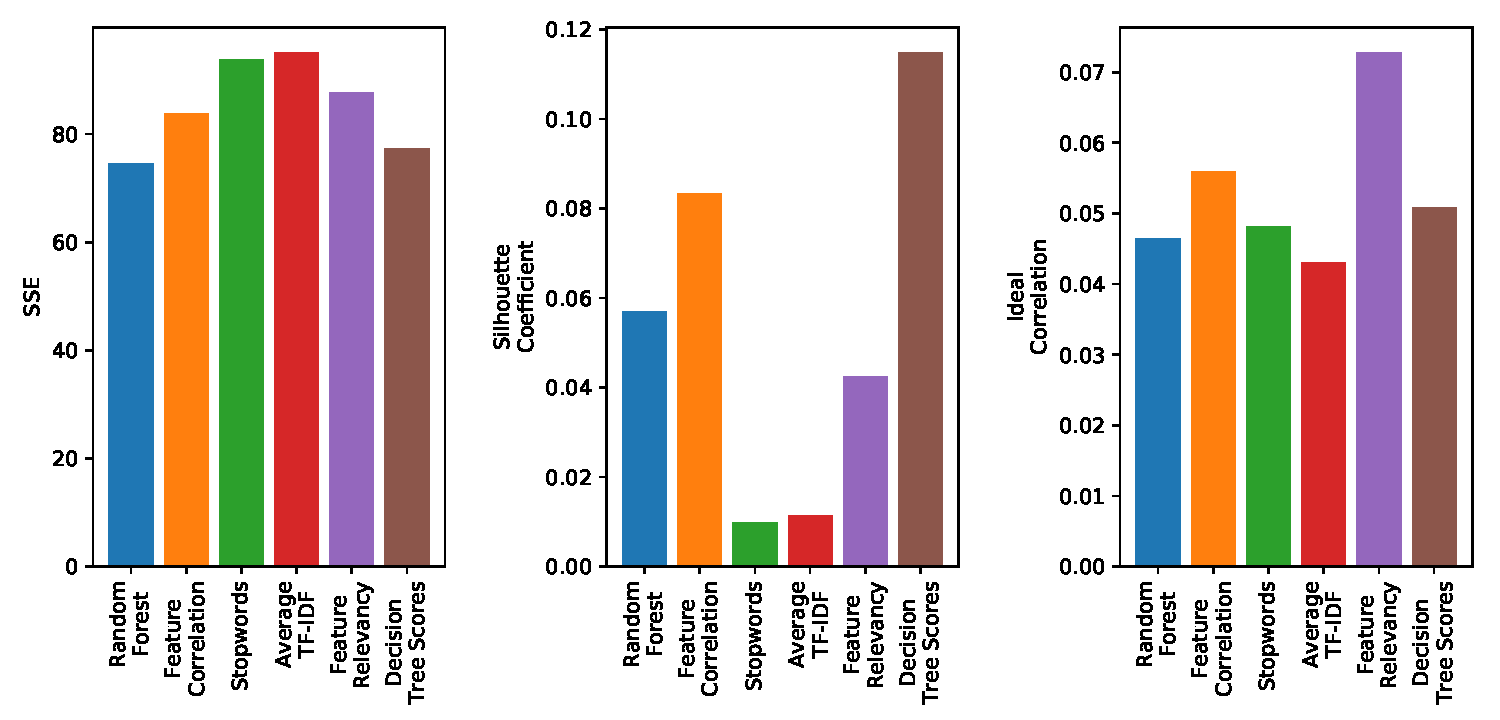
\includegraphics[height=0.3\textheight]{figures/hw3/euclidean/feature_subset_selection}
  \caption{With Euclidean distance as the distance metric for $k$-means clustering, the method for feature subset selection as was varied to observe the effects on the resulting clustering's SSE, silhouette coefficient, and ideal-class/cluster similarity matrix correlation.}
\end{figure}

\begin{figure} \label{fig:something}
  \centering
  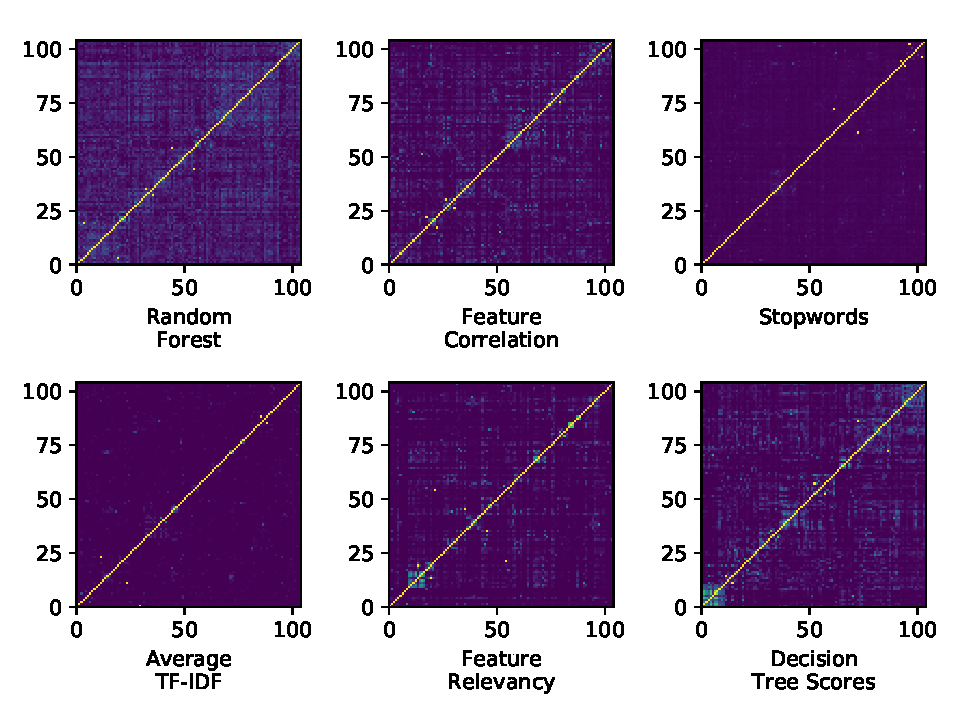
\includegraphics[width=0.9\textwidth]{figures/hw3/euclidean/similarity_matrices}
  \caption{With Euclidean distance as the distance metric for $k$-means clustering, the method for feature subset selection as was varied to observe the effects on the resulting similarities between articles within each cluster.}
\end{figure}


\subsection{$k$-means on Cosine Distance}

%figures/hw3/cosine/feature_subset_selection
%figures/hw3/cosine/natural_clusters
%figures/hw3/cosine/similarity_matrices

\begin{figure}[h!] \label{fig:something}
  \centering
  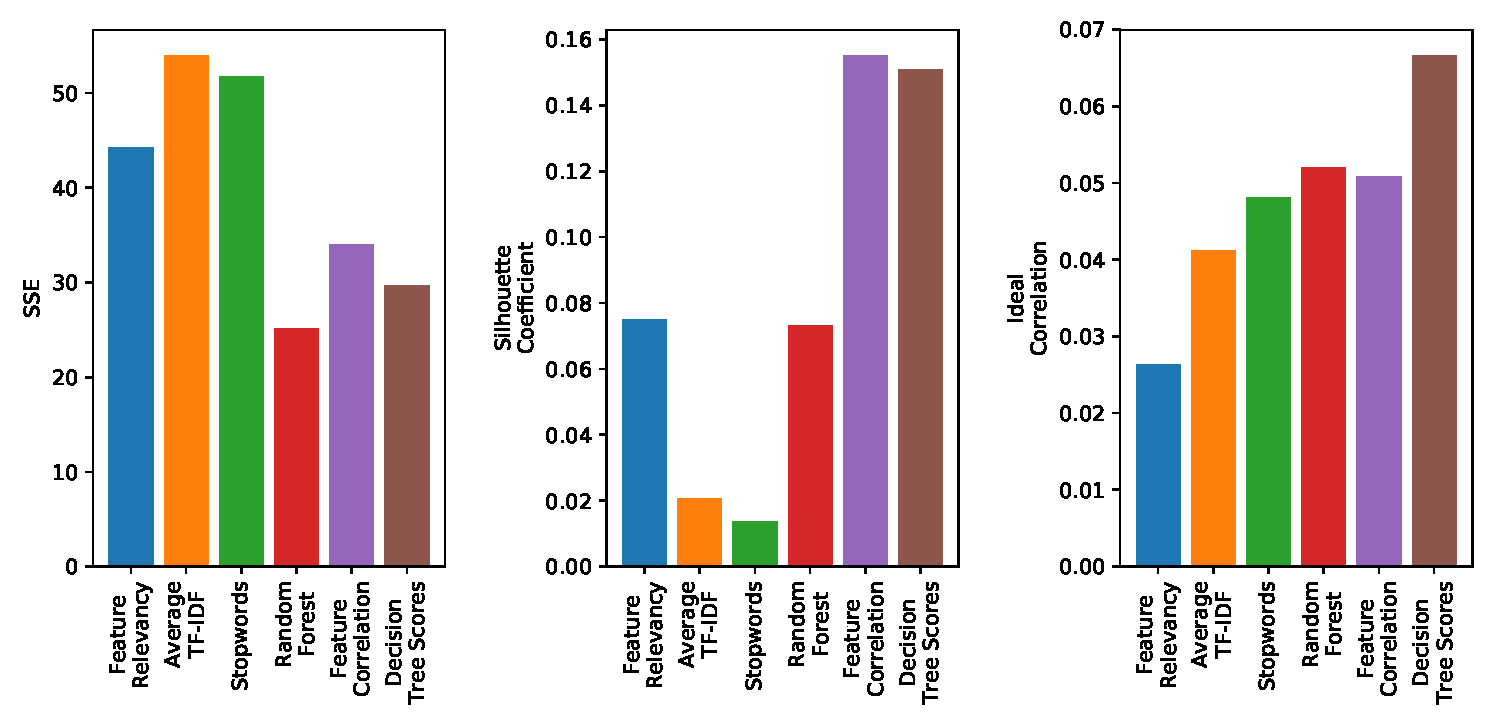
\includegraphics[height=0.3\textheight]{figures/hw3/cosine/feature_subset_selection}
  \caption{With Cosine distance as the distance metric for $k$-means clustering, the method for feature subset selection as was varied to observe the effects on the resulting clustering's SSE, silhouette coefficient, and ideal-class/cluster similarity matrix correlation.}
\end{figure}

\begin{figure}[h!] \label{fig:something}
  \centering
  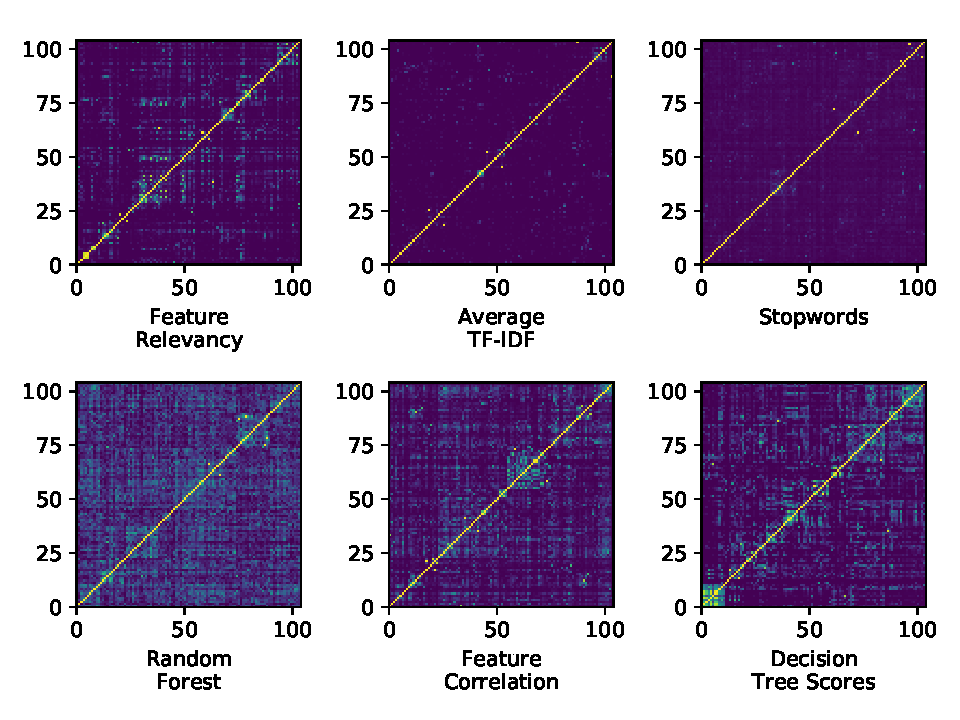
\includegraphics[width=0.9\textwidth]{figures/hw3/cosine/similarity_matrices}
  \caption{With Cosine distance as the distance metric for $k$-means clustering, the method for feature subset selection as was varied to observe the effects on the resulting similarities between articles within each cluster.}
\end{figure}

With the cosine distance being used in $k$-means, it is again observed in Figure 3 that both the feature selection based on average tf-idf scores and the removal of stopwords continues to perform poorly, with higher SSEs and lower silhouette coefficients.
However, contrary to its performance under Euclidean distance, the feature relevancy based method drops in its ability to produce higher quality clusters.
Instead, the decision tree based method for feature selection performs the best out of methods tested, offering more cohesive and better separated (by its higher silhouette coefficient), and closer to ideal clusters (by its ideal class/cluster matrix correlation).
This can further be seen by observing the better-defined structures in its similarity matrix in Figure 4.

It is also worth mentioning that the feature correlation method and the random forest method also offer better similarity matrices and more compact clusters, but their effectiveness in producing class-based clusters is noticeably less than that of the decision tree method.

However, as was the case in the previous section, the results presented here still suggest that the produced clusters are not suitable for classification.
Even with the decision tree-based feature selection method offering the best correlation between its ideal cluster and ideal class similarity matrices, the resulting correlation falls below that of the previous section at approximately 0.067.


\subsection{$k$-means on the Jaccard Distance}

With the Jaccard distance used for $k$-means, the resulting performance is significantly poor across every method.
From Figure 5, it is observed that the clusters produced from every feature selection method are nearly equal in terms of their SSEs.
Again, stopword removal and average tf-idf based feature selection methods have the worst silhouette coefficients, this time equal to 0, implying that the articles within each cluster are about as close to articles in other clusters as they are in their own.
This can be also observed in Figure 6, where there is no discernable pattern in any of the similarity matrices of each method.
Ultimately, this suggests that the Jaccard distance metric is not suitable for $k$-means clustering on a tf-idf representation of articles, as well determined in the previous report.

\begin{figure}[h!] \label{fig:something}
  \centering
  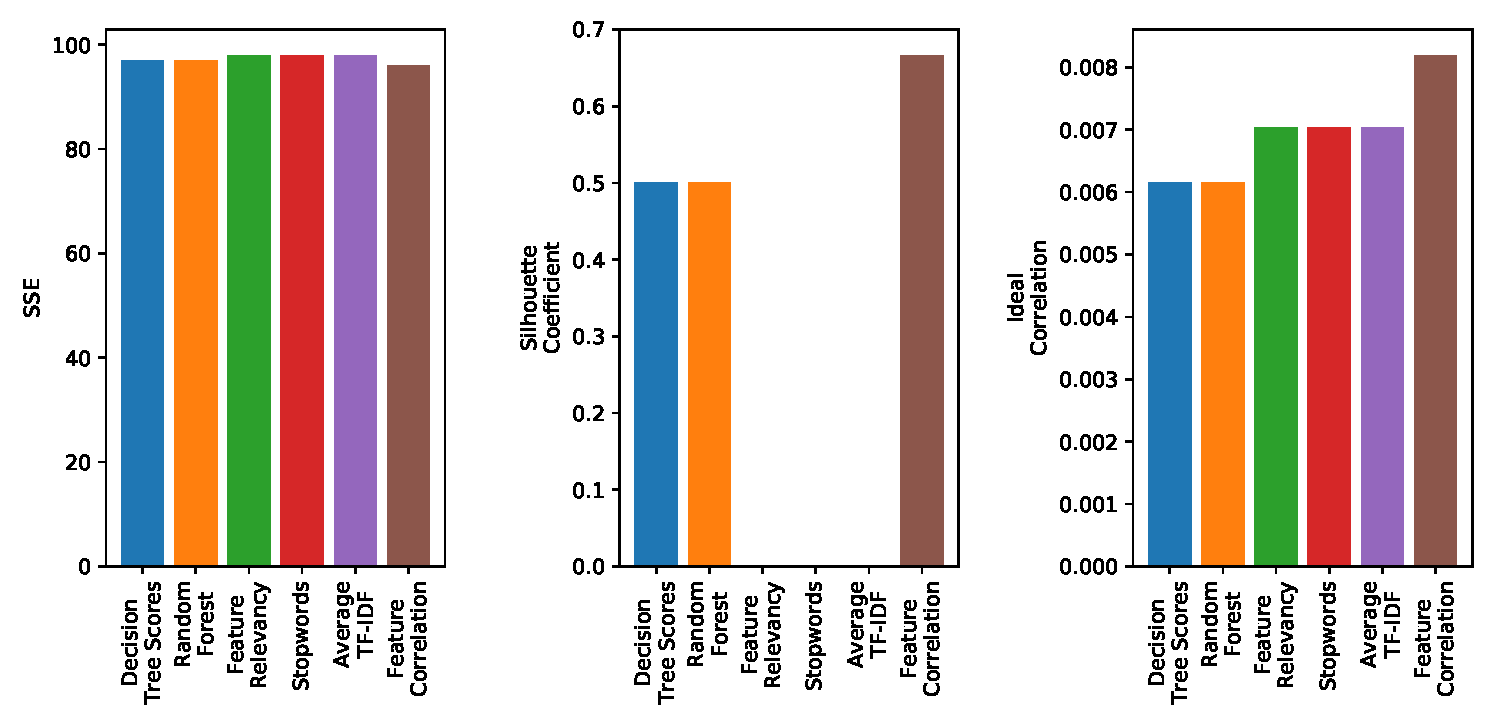
\includegraphics[width=\textwidth]{figures/hw3/jaccard/feature_subset_selection}
  \caption{With Jaccard distance as the distance metric for $k$-means clustering, the method for feature subset selection as was varied to observe the effects on the resulting clustering's SSE, silhouette coefficient, and ideal-class/cluster similarity matrix correlation.}
\end{figure}

\begin{figure}[h!] \label{fig:something}
  \centering
  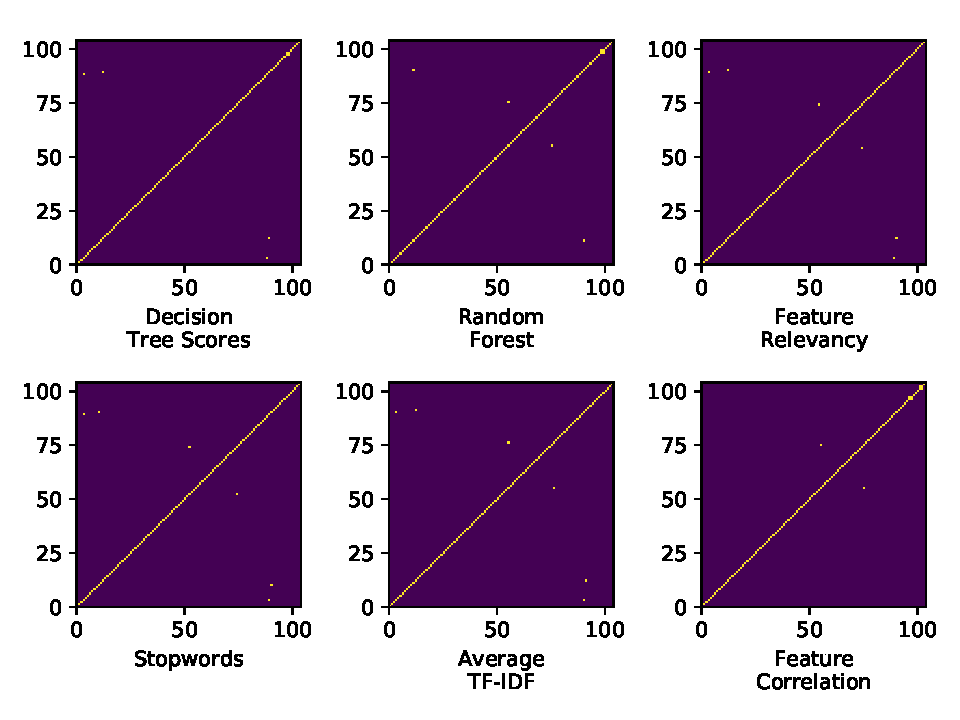
\includegraphics[width=\textwidth]{figures/hw3/jaccard/similarity_matrices}
  \caption{With Jaccard distance as the distance metric for $k$-means clustering, the method for feature subset selection as was varied to observe the effects on the resulting similarities between articles within each cluster.}
\end{figure}


%figures/hw3/jaccard/feature_subset_selection
%figures/hw3/jaccard/natural_clusters
%figures/hw3/jaccard/similarity_matrices

\subsection{Investigating Natural Clusters}

Ideally, the result of a clustering should produce clusters that contain only articles of a particular category.
In the above experiments, the number of clusters constructed by the $k$-means algorithm was equal to the number of article categories.
The results from these experiments indicated that clustering in this manner, under the tested preprocessing methods and distance metrics, could not produce clusters exhibiting a high purity in the classes of articles contained in them.
Because of this, one additional set of experiments was conducted to observe the properties of the clusters produced when the number of clusters was allowed to increase.
For these experiments, the feature-to-class relevancy based method was chosen for feature selection of the dataset during preprocessing, as it was suggested to be the best performing method overall based on the findings in Section \ref{sec:euclid}.

The motivation behind this additional set of experiments is based on the intuition that, although the articles may not be effectively clustered into 7 clusters, there may exist a natural clustering of the articles that results in each cluster being significantly pure in regards to the categories of the articles within each cluster.
Naturally, this can only occur if the dataset is clustered into 7 or more clusters.
With this intuition, a set of experiments was conducted to observe the overall SSE, silhoette coefficient, and the average purity of the clusters resulting from $k$ increasing beyond 7.
The results of these experiences are shown in Figure 6.

From Figure 6, it can be observed that an increase in the number of clusters results in lower SSEs and in increasing silhouette coefficients and average cluster purity.
Because there are more clusters, the SSE of each cluster is expected to decrease because of the centroid-based nature of the $k$-means algorithms.
However, with the silhouette coefficient, there are peaks at $k = 7$ when using the Euclidean distance, and at $k = 9$ and $17$ when using cosine distances.
This suggests that the clusterings produced at those $k$-values are better separated and more cohesive than the clusterings produced by immediately lower and higher $k$ values.
By also observing the average cluster purity, there is a mild peak that occurs at $k = 17$ as well, suggesting that permitting 17 clusters can produce clusters of reduced contamination.
However, they still are not signficantly pure so as to be useful in classification.
Due to the small sample size of the dataset, $k$-values higher than 21 produced many singleton clusters, rendering the experimental analysis on those clusterings less meaningful.
Unfortunately, due to time constraints, a more thorough analysis with a larger dataset was not possible at this time.


\begin{figure}[h!] \label{fig:something}
  \centering
  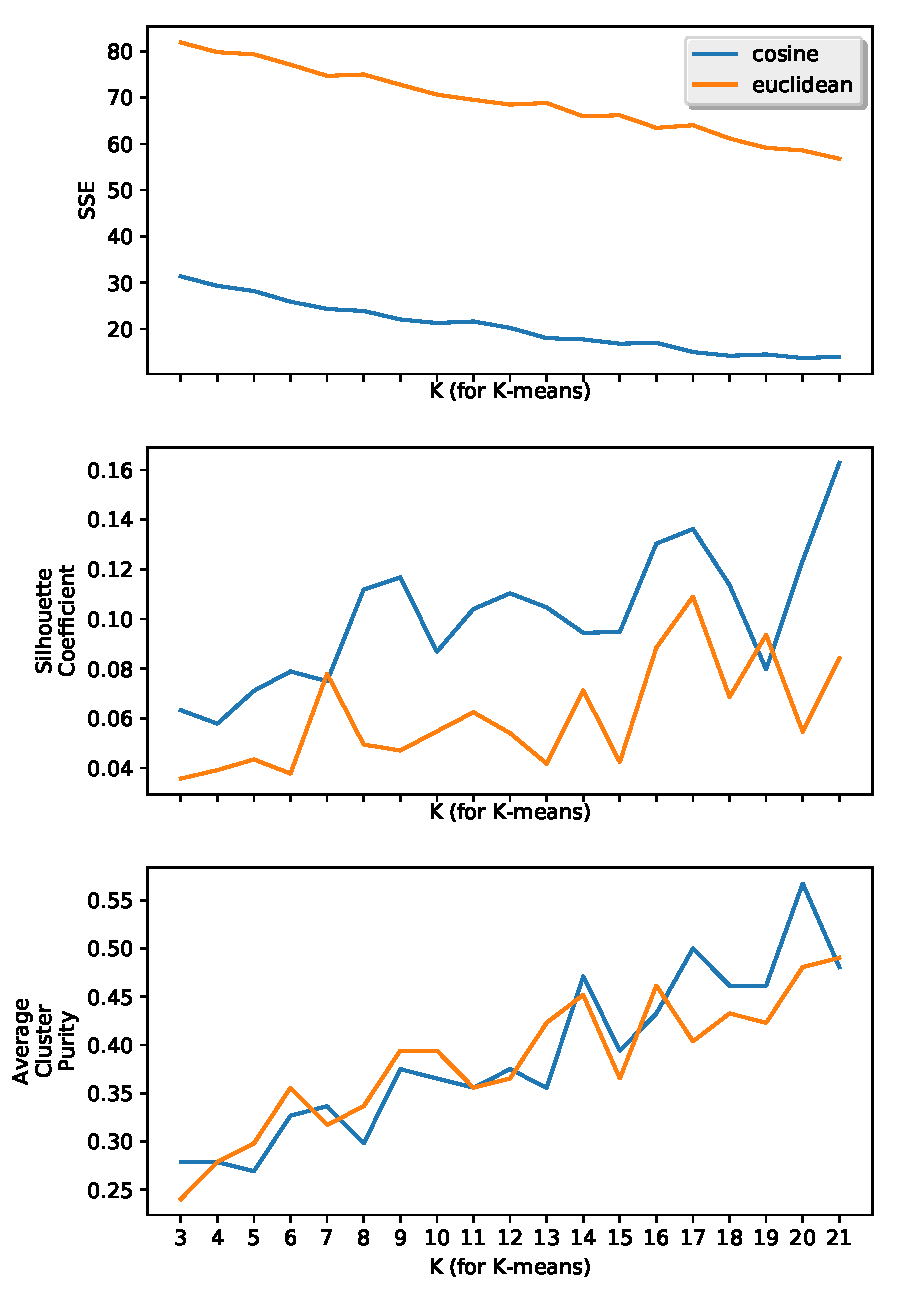
\includegraphics[height=0.6\textheight]{figures/hw3/natural_clusters}
  \caption{When the number of clusters to be found by $k$-means is allowed to increase, the resulting SSE, silhouette coefficients, and average cluster purity is observed to investigate whether there exists a natural clustering of the articles that produces pure category-based clusters.}
\end{figure}

%\begin{figure}[h!] \label{fig:something}
%  \centering
%  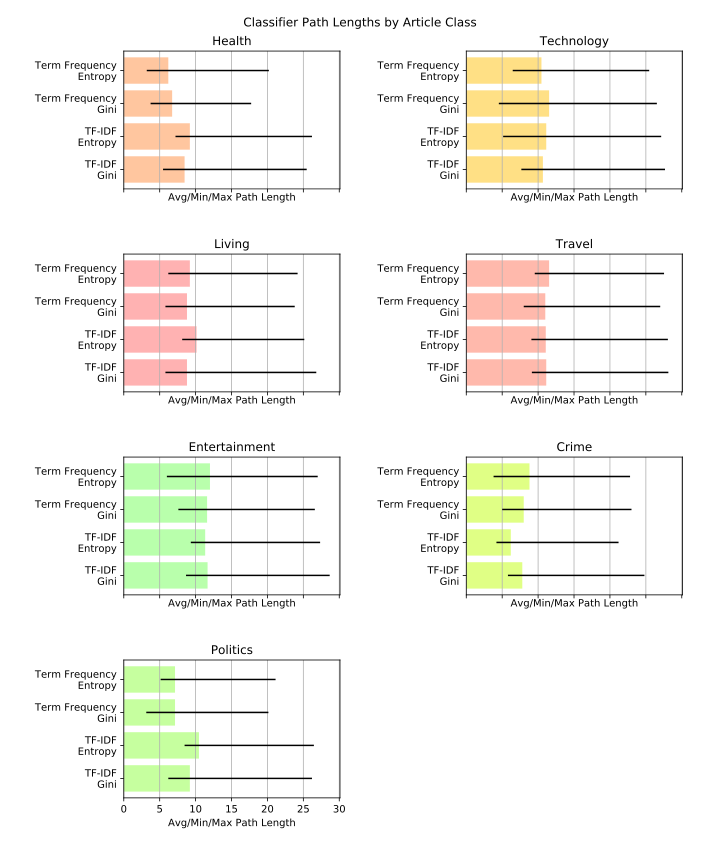
\includegraphics[width=\textwidth]{figures/decision_tree/mrmr/path_depths}
%  \caption{}
%\end{figure}

%\begin{figure}[h!] \label{fig:somethingelse}
%	\centering
%	\begin{subfigure}{.5\textwidth}
%	  \centering
%	  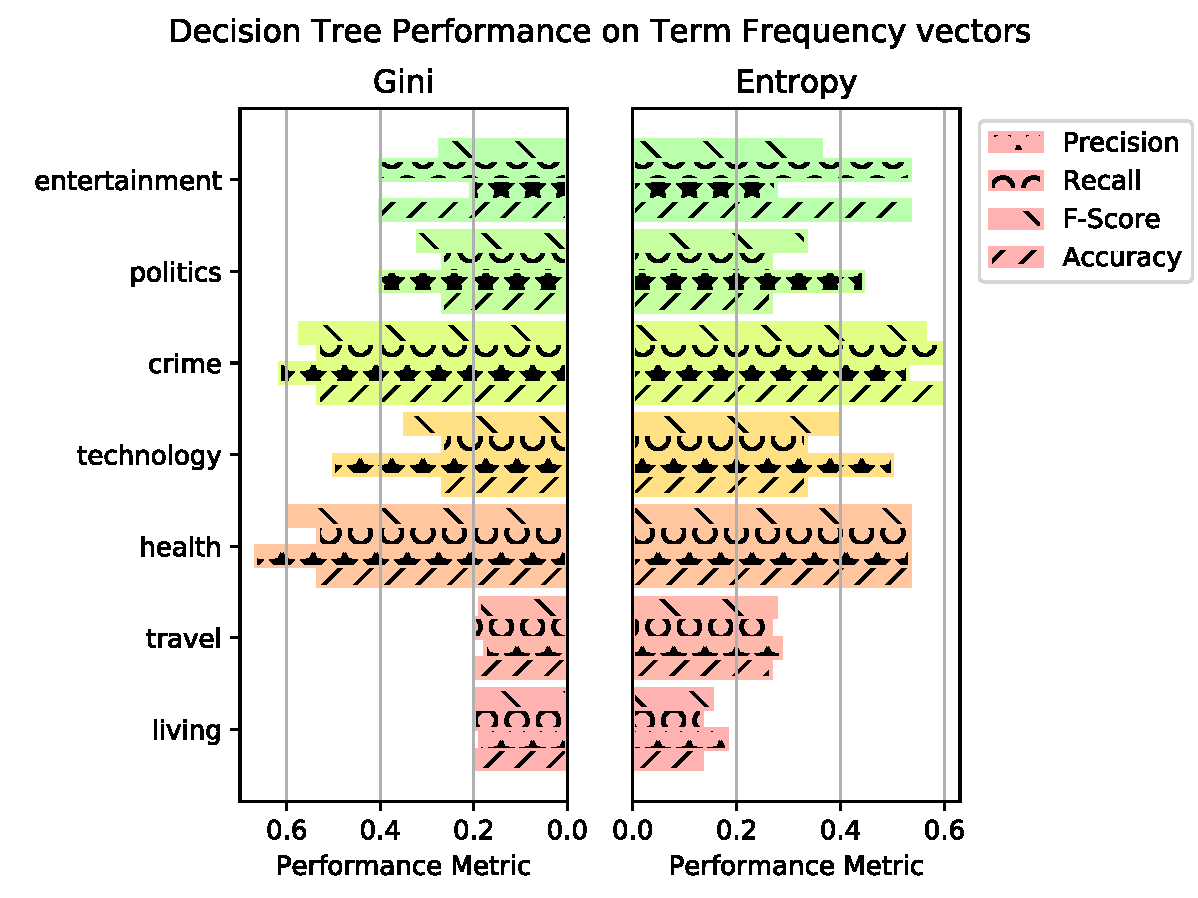
\includegraphics[width=\linewidth]{figures/decision_tree/tf_prec_n_rec}
%	  \caption{}
%	\end{subfigure}%
%	\begin{subfigure}{.5\textwidth}
%	  \centering
%	  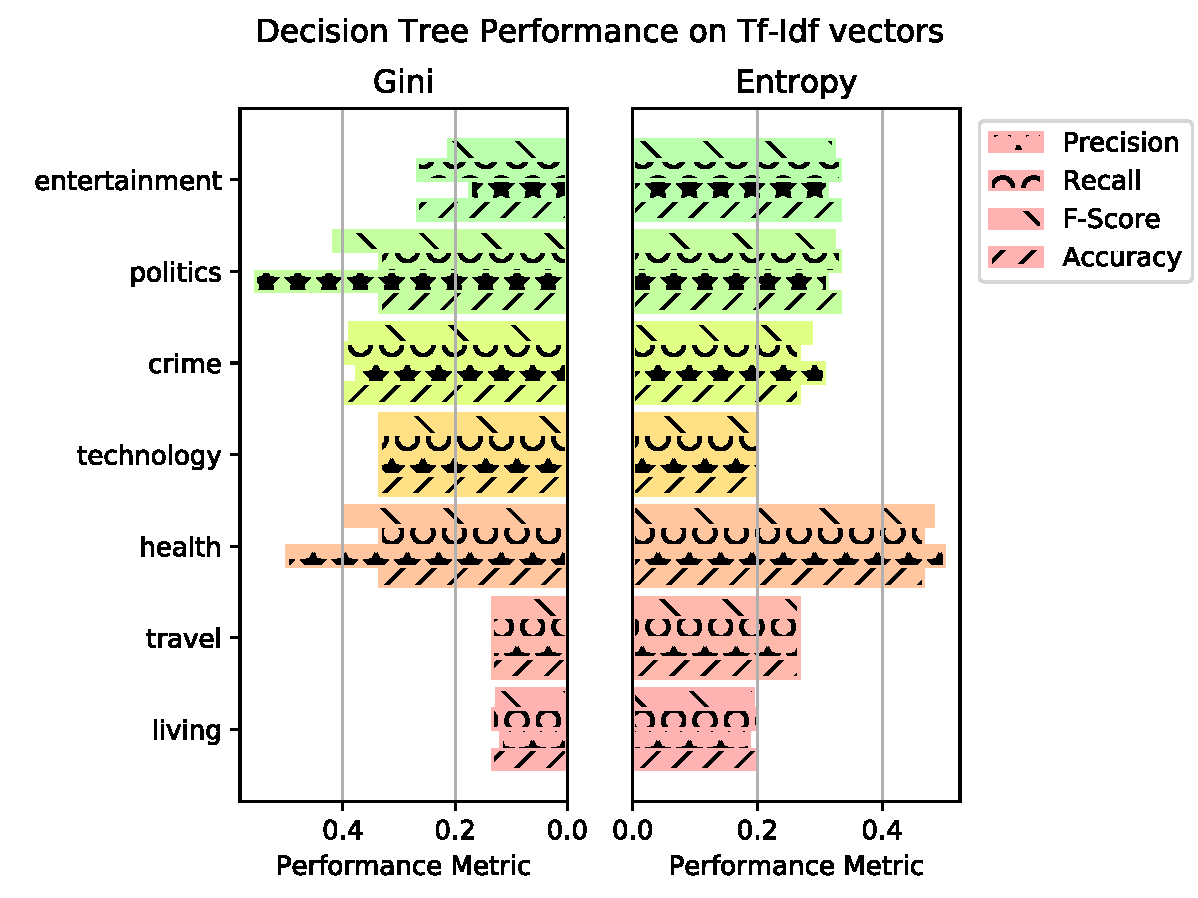
\includegraphics[width=\linewidth]{figures/decision_tree/tfidf_prec_n_rec}
%	  \caption{}
%	\end{subfigure}
%	\caption{}
%\end{figure}


\section{Conclusion}

From the above experiments, it is suggested that performing feature selection as a preprocessing step is necessary to improve the results of $k$-means clustering on a dataset of news articles.
Of the tested feature selection methods, the feature-to-class relevancy based method and the decision tree-based method offered better preprocessed datasets when fed into the $k$-means algorithm.
The clusters resulting from these datasets exhibited better compactness and separation, along with a higher correlation to an ideal clustering defined by article categories.
However, these clusters were found to be insufficient for performing classification on the articles.
In terms of distance metrics, the Euclidean distance performed slightly better than the cosine distance with regards to the same ideal clustering correlation.
Ultimately, the findings of this report suggest that clustering cannot be used as a single method for classification, but rather may be useful if integrated into a much larger ensemble of classification and clustering strategies.

\bibliography{bibliography}{}
\bibliographystyle{plain}
\end{document}